\documentclass[10pt]{beamer}\usepackage[]{graphicx}\usepackage[]{color}
%% maxwidth is the original width if it is less than linewidth
%% otherwise use linewidth (to make sure the graphics do not exceed the margin)
\makeatletter
\def\maxwidth{ %
  \ifdim\Gin@nat@width>\linewidth
    \linewidth
  \else
    \Gin@nat@width
  \fi
}
\makeatother

\definecolor{fgcolor}{rgb}{0.345, 0.345, 0.345}
\newcommand{\hlnum}[1]{\textcolor[rgb]{0.686,0.059,0.569}{#1}}%
\newcommand{\hlstr}[1]{\textcolor[rgb]{0.192,0.494,0.8}{#1}}%
\newcommand{\hlcom}[1]{\textcolor[rgb]{0.678,0.584,0.686}{\textit{#1}}}%
\newcommand{\hlopt}[1]{\textcolor[rgb]{0,0,0}{#1}}%
\newcommand{\hlstd}[1]{\textcolor[rgb]{0.345,0.345,0.345}{#1}}%
\newcommand{\hlkwa}[1]{\textcolor[rgb]{0.161,0.373,0.58}{\textbf{#1}}}%
\newcommand{\hlkwb}[1]{\textcolor[rgb]{0.69,0.353,0.396}{#1}}%
\newcommand{\hlkwc}[1]{\textcolor[rgb]{0.333,0.667,0.333}{#1}}%
\newcommand{\hlkwd}[1]{\textcolor[rgb]{0.737,0.353,0.396}{\textbf{#1}}}%
\let\hlipl\hlkwb

\usepackage{framed}
\makeatletter
\newenvironment{kframe}{%
 \def\at@end@of@kframe{}%
 \ifinner\ifhmode%
  \def\at@end@of@kframe{\end{minipage}}%
  \begin{minipage}{\columnwidth}%
 \fi\fi%
 \def\FrameCommand##1{\hskip\@totalleftmargin \hskip-\fboxsep
 \colorbox{shadecolor}{##1}\hskip-\fboxsep
     % There is no \\@totalrightmargin, so:
     \hskip-\linewidth \hskip-\@totalleftmargin \hskip\columnwidth}%
 \MakeFramed {\advance\hsize-\width
   \@totalleftmargin\z@ \linewidth\hsize
   \@setminipage}}%
 {\par\unskip\endMakeFramed%
 \at@end@of@kframe}
\makeatother

\definecolor{shadecolor}{rgb}{.97, .97, .97}
\definecolor{messagecolor}{rgb}{0, 0, 0}
\definecolor{warningcolor}{rgb}{1, 0, 1}
\definecolor{errorcolor}{rgb}{1, 0, 0}
\newenvironment{knitrout}{}{} % an empty environment to be redefined in TeX

\usepackage{alltt}%
\usetheme{Boadilla}
\usecolortheme{seahorse}

\usepackage[utf8]{inputenc}%

% graphics
%% Figures %%%%%%%%%%%%%%%%%%%%%%%%%%%%%%%%%%%%%%%%%%%%%%%%%%
\usepackage{graphicx}
\usepackage{xcolor}%for color mixing

\usepackage{amsmath}%
\usepackage{amsfonts}%
\usepackage{amssymb}%
\usepackage{graphicx}

\usepackage{tikz}

%%%%%%%%%%%%%%%%%%%%%%%%%%%%%%%%%%%%%%%%%%%%%%
%%%%%%%%%%%%%%%%% Doc info %%%%%%%%%%%%%%%%%%%
\title[\textbf{Linear models}]{Statistical inference and linear models}
\date{\today}

%%%%%%%%%%%%%%%%%%%%%%%%%%%%%%%%%%%%
\IfFileExists{upquote.sty}{\usepackage{upquote}}{}
\begin{document}
%\SweaveOpts{concordance=TRUE}




\begin{frame}
\maketitle	
\end{frame}
%%%%%%%%%%%

\AtBeginSection[]
{
  \begin{frame}<beamer>
    \frametitle{}
    \tableofcontents[currentsection,hideothersubsections,subsectionstyle=hide]% down vote\tableofcontents[currentsection,currentsubsection,hideothersubsections,sectionstyle=show/hide,subsectionstyle=show/shaded/hide] 
  \end{frame}
} 


\section{Statistical inference}%very general, still simplistic

\begin{frame}{General approach}

\begin{center}
  \begin{tikzpicture}
    \node (sq) at (0,-1) {\color{red}{1. Scientific question}};
    \pause
    \node (mo) at (0,-2) {2. Model and Statistical question};
    \draw[->, thick] (sq)--(mo);
    \pause
    \node (dac) at (6,-2) {\color{red}{3. Data collection}};
    \draw[<->, thick] (mo)--(dac);
    \pause
    \node (est) at (0,-3) {4.a Estimation};
        \draw[->, thick] (mo)--(est);
    \node (unc) at (0,-3.5) {4.b Uncertainty and statistical significance};
    \pause
    
    \node (che) at (0,-5) {5. Diagnostic, check assumptions, prediction};
        \draw[->, thick] (unc)--(che);
    \draw[->, thick] (che.west) to [out=150, in=210] (mo.west);

    \pause
    \node (int) at (0,-6) {\color{red}{6. Interpret and think about the biology}};
        \draw[->, thick] (che)--(int);

  \draw[rounded corners, color=blue] (-4.5,-1.5) rectangle (4,-5.5);
  \node[anchor=north west] (r) at (-4.5,-1.5) {
\includegraphics[width=0.1\textwidth]{Figures/r}};
  \end{tikzpicture}
  \end{center}
\end{frame}
%%%%%%%%%%%

\begin{frame}[fragile]{Iris t.test}
  
  \pause
\begin{knitrout}
\definecolor{shadecolor}{rgb}{0.843, 0.867, 0.922}\color{fgcolor}\begin{kframe}
\begin{alltt}
  \hlkwd{data}\hlstd{(}\hlstr{"iris"}\hlstd{)}
\end{alltt}
\end{kframe}
\end{knitrout}

\begin{knitrout}
\definecolor{shadecolor}{rgb}{0.843, 0.867, 0.922}\color{fgcolor}\begin{kframe}
\begin{alltt}
  \hlkwd{str}\hlstd{(iris)}
  \hlkwd{plot}\hlstd{(iris)}
\end{alltt}
\end{kframe}
\end{knitrout}
  
  \begin{enumerate}
    \item \color{red}{Scientific question}: Are the taxa "setosa" and "versicolor" different species?
  \pause
    \item Model and stat question:
      \begin{itemize}
        \item Model:
          \begin{itemize}
            \item There is an intrinsic/expected sepal length value for a species; an individual value is the sum of this expectation and a random Gaussian deviation.
            \item $y_i = \mu_{species_i} + \epsilon_i$ with  $\epsilon \sim N(0,\sigma^2)$
            \item t-test
          \end{itemize}
        \pause
        \item Statistical question: 
          \begin{itemize}
            \item Does sepal length \textbf{differ significantly} between the two taxa \textbf{in our sample}?
            \item Is the observed difference between taxa likely if both taxa have the same intrinsic/expected value?
          \end{itemize}
        \end{itemize}
      \item Data collection
    \end{enumerate}
\end{frame}
%%%%%%%%%%%

\begin{frame}[fragile]{Iris t.test, visualization}
\centering
\begin{knitrout}
\definecolor{shadecolor}{rgb}{0.843, 0.867, 0.922}\color{fgcolor}\begin{kframe}
\begin{alltt}
\hlkwd{boxplot}\hlstd{(Sepal.Length} \hlopt{~} \hlstd{Species,}
        \hlkwc{data} \hlstd{= iris[iris}\hlopt{$}\hlstd{Species} \hlopt \hlkwd{c}\hlstd{(}\hlstr{"setosa"}\hlstd{,}\hlstr{"versicolor"}\hlstd{),],}
        \hlkwc{drop} \hlstd{=} \hlnum{TRUE}\hlstd{,} \hlkwc{ylab}\hlstd{=}\hlstr{"Sepal length"}\hlstd{,} \hlkwc{xlab}\hlstd{=}\hlstr{"Species"}\hlstd{)}
\end{alltt}
\end{kframe}
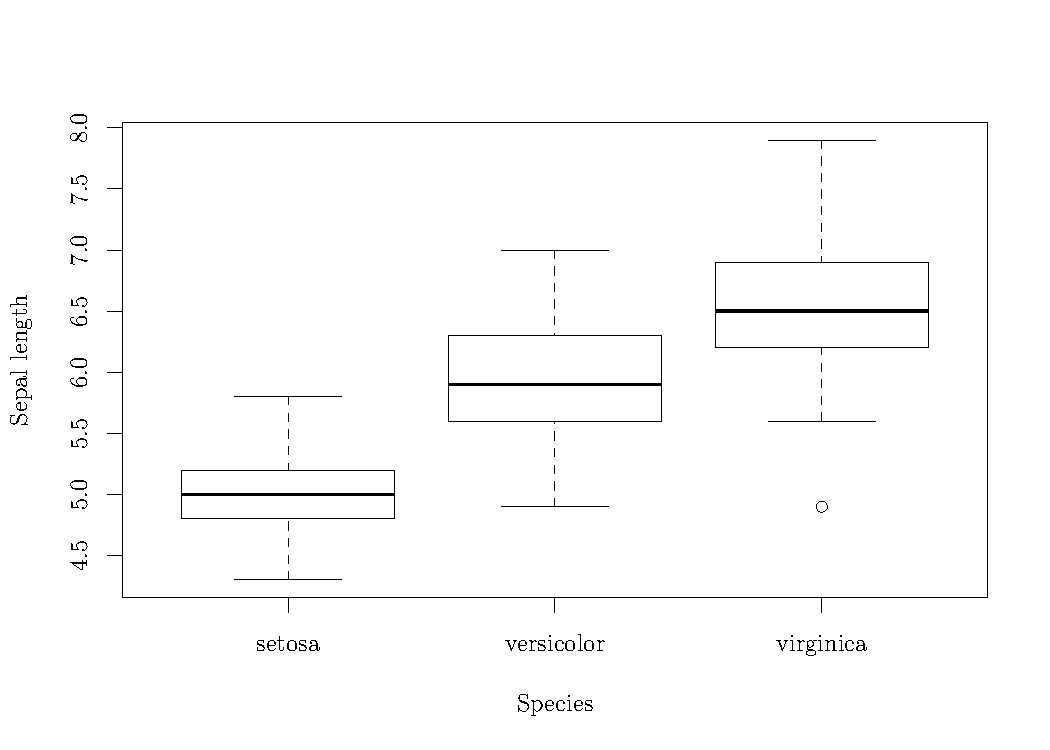
\includegraphics[width=0.7\textwidth,height=0.5\textwidth]{figure/boxplot-1} 

\end{knitrout}
\end{frame}
%%%%%%%%%%%


\begin{frame}[fragile]{Iris t.test, visualization}
\centering
\begin{knitrout}
\definecolor{shadecolor}{rgb}{0.843, 0.867, 0.922}\color{fgcolor}\begin{kframe}
\begin{alltt}
\hlkwd{library}\hlstd{(ggplot2)}
  \hlkwd{ggplot}\hlstd{( iris[iris}\hlopt{$}\hlstd{Species} \hlopt \hlkwd{c}\hlstd{(}\hlstr{"setosa"}\hlstd{,}\hlstr{"versicolor"}\hlstd{),],}
          \hlkwd{aes}\hlstd{(}\hlkwc{x}\hlstd{=Species,} \hlkwc{y}\hlstd{=Sepal.Length))} \hlopt{+} \hlkwd{geom_boxplot}\hlstd{()}
\end{alltt}
\end{kframe}
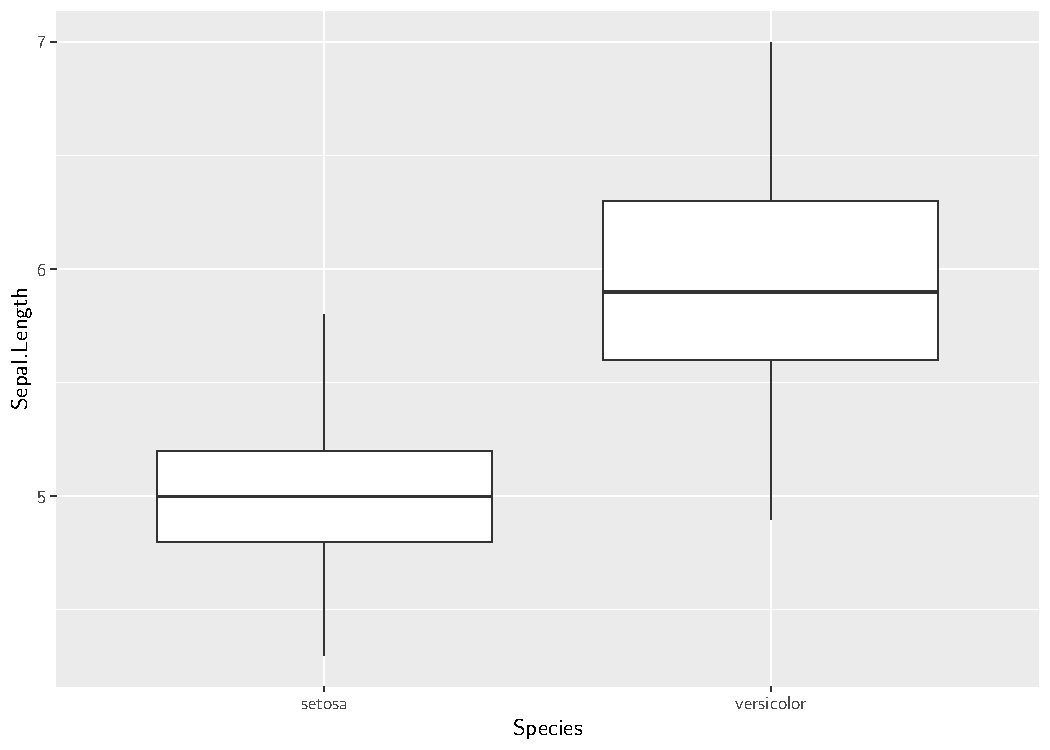
\includegraphics[width=0.7\textwidth,height=0.5\textwidth]{figure/ggboxplot-1} 

\end{knitrout}
\end{frame}
%%%%%%%%%%%


\begin{frame}[fragile]{Iris t.test}
    One t-test for sepal length between \textit{setosa} and \textit{versicolor}:
\begin{knitrout}
\definecolor{shadecolor}{rgb}{0.843, 0.867, 0.922}\color{fgcolor}\begin{kframe}
\begin{alltt}
  \hlkwd{t.test}\hlstd{(}\hlkwc{x} \hlstd{= iris}\hlopt{$}\hlstd{Sepal.Length[iris}\hlopt{$}\hlstd{Species} \hlopt{==} \hlstr{"setosa"}\hlstd{],}
        \hlkwc{y} \hlstd{= iris}\hlopt{$}\hlstd{Sepal.Length[iris}\hlopt{$}\hlstd{Species} \hlopt{==} \hlstr{"versicolor"}\hlstd{])}
\end{alltt}
\begin{verbatim}

	Welch Two Sample t-test

data:  iris$Sepal.Length[iris$Species == "setosa"] and iris$Sepal.Length[iris$Species == "versicolor"]
t = -10.521, df = 86.538, p-value < 2.2e-16
alternative hypothesis: true difference in means is not equal to 0
95 percent confidence interval:
 -1.1057074 -0.7542926
sample estimates:
mean of x mean of y 
    5.006     5.936 
\end{verbatim}
\end{kframe}
\end{knitrout}
  
\end{frame}
%%%%%%%%%%%

\begin{frame}[fragile]{When do we know it is different?}

\begin{enumerate}
  \setcounter{enumi}{3}
  \item Statistical estimation
  \begin{itemize}
    \item a Estimation
      \begin{itemize}
        \item Cannot know true difference $\mu_{species_1} - \mu_{species_2}$
        \item Estimated difference $= \color{red}{\text{Mean}_1 - \text{Mean}_2 }$
        \item Estimated difference contains random variation
      \end{itemize}
    \item b Quantify uncertainty / Statistical significance
      \begin{itemize}
        \item $
      t = \frac{\color{red}{\text{Mean}_1 - \text{Mean}_2}}{\text{\color{orange}Variation}}
      \frac{\sqrt{{\text{\color{blue}{Sample Size}}}}}{\sqrt{2}}
      $
        \item We know exactly how t is distributed when $\mu_{species_1} - \mu_{species_2} = 0$
        \item Hence we know probability of $\geq t$ if $\mu_{species_1} - \mu_{species_2} = 0$ ($p$-value)
        \item Can derive confidence interval and standard error
      \end{itemize}
  \end{itemize}
\end{enumerate}

\pause
Less uncertainty with
  \begin{itemize}
    \item \color{red}{Larger absolute difference}
    \item \color{orange}{Smaller variability}
    \item \color{blue}{Larger sample size}
  \end{itemize}


\end{frame}
%%%%%%%%%%%

\begin{frame}[fragile]{When do we know it is different? Simulations}

\begin{block}{Simulations in R}
  \begin{itemize}
    \item Pseudo-random generator
    \item Deterministic chain starting from a number calculated from computer time and R processus ID (the "seed")
    \item Hence reproducible using \texttt{set.seed()}
    \item Default algorithm: Mersenne-Twister
  \end{itemize}

\begin{knitrout}
\definecolor{shadecolor}{rgb}{0.843, 0.867, 0.922}\color{fgcolor}\begin{kframe}
\begin{alltt}
  \hlkwd{rnorm}\hlstd{(}\hlkwc{n} \hlstd{= ,} \hlkwc{mean} \hlstd{= ,} \hlkwc{sd} \hlstd{= )}
\end{alltt}
\end{kframe}
\end{knitrout}

\end{block}

\end{frame}
%%%%%%%%%%%
  
\begin{frame}[fragile]{When do we know it is different? Simulations}
\pause
\textbf{\color{red}{1. Larger absolute difference}}
\begin{knitrout}
\definecolor{shadecolor}{rgb}{0.843, 0.867, 0.922}\color{fgcolor}\begin{kframe}
\begin{alltt}
\hlstd{nbsim} \hlkwb{<-} \hlnum{1000}
\hlstd{pdistri_large} \hlkwb{<-} \hlkwd{vector}\hlstd{(}\hlkwc{length} \hlstd{= nbsim)}
\hlstd{pdistri_small} \hlkwb{<-} \hlkwd{vector}\hlstd{(}\hlkwc{length} \hlstd{= nbsim)}
\hlkwa{for} \hlstd{(i} \hlkwa{in} \hlnum{1}\hlopt{:}\hlstd{nbsim)}
  \hlstd{\{}
  \hlstd{x1} \hlkwb{<-} \hlkwd{rnorm}\hlstd{(}\hlkwc{n} \hlstd{=} \hlnum{10}\hlstd{,} \hlkwc{mean} \hlstd{=} \hlnum{2}\hlstd{,} \hlkwc{sd} \hlstd{=} \hlnum{1}\hlstd{)}
  \hlstd{x2} \hlkwb{<-} \hlkwd{rnorm}\hlstd{(}\hlkwc{n} \hlstd{=} \hlnum{10}\hlstd{,} \hlkwc{mean} \hlstd{=} \hlnum{4}\hlstd{,} \hlkwc{sd} \hlstd{=} \hlnum{1}\hlstd{)} \hlcom{#large diff}
  \hlstd{x3} \hlkwb{<-} \hlkwd{rnorm}\hlstd{(}\hlkwc{n} \hlstd{=} \hlnum{10}\hlstd{,} \hlkwc{mean} \hlstd{=} \hlnum{2.5}\hlstd{,} \hlkwc{sd} \hlstd{=} \hlnum{1}\hlstd{)} \hlcom{#small diff}
  \hlstd{out_large} \hlkwb{<-} \hlkwd{t.test}\hlstd{(x1, x2)}
  \hlstd{out_small} \hlkwb{<-} \hlkwd{t.test}\hlstd{(x1, x3)}
  \hlstd{pdistri_large[i]}\hlkwb{<-}\hlstd{out_large}\hlopt{$}\hlstd{p.value}
  \hlstd{pdistri_small[i]}\hlkwb{<-}\hlstd{out_small}\hlopt{$}\hlstd{p.value}
\hlstd{\}}
\end{alltt}
\end{kframe}
\end{knitrout}
\end{frame}
%%%%%%%%%%
\begin{frame}[fragile]{When do we know it is different?}
\centering
\begin{knitrout}
\definecolor{shadecolor}{rgb}{0.843, 0.867, 0.922}\color{fgcolor}\begin{kframe}
\begin{alltt}
\hlkwd{par}\hlstd{(}\hlkwc{mfrow}\hlstd{=}\hlkwd{c}\hlstd{(}\hlnum{1}\hlstd{,}\hlnum{2}\hlstd{),} \hlkwc{cex}\hlstd{=}\hlnum{2}\hlstd{)}
\hlkwd{hist}\hlstd{(pdistri_large,} \hlkwc{xlim}\hlstd{=}\hlkwd{c}\hlstd{(}\hlnum{0}\hlstd{,}\hlnum{1}\hlstd{),}
     \hlkwc{main}\hlstd{=}\hlkwd{paste}\hlstd{(}\hlstr{"Prop signif="}\hlstd{,}\hlkwd{mean}\hlstd{(pdistri_large}\hlopt{<}\hlnum{0.05}\hlstd{)))}
\hlkwd{hist}\hlstd{(pdistri_small,} \hlkwc{xlim}\hlstd{=}\hlkwd{c}\hlstd{(}\hlnum{0}\hlstd{,}\hlnum{1}\hlstd{),}
     \hlkwc{main}\hlstd{=}\hlkwd{paste}\hlstd{(}\hlstr{"Prop signif="}\hlstd{,}\hlkwd{mean}\hlstd{(pdistri_small}\hlopt{<}\hlnum{0.05}\hlstd{)))}
\end{alltt}
\end{kframe}
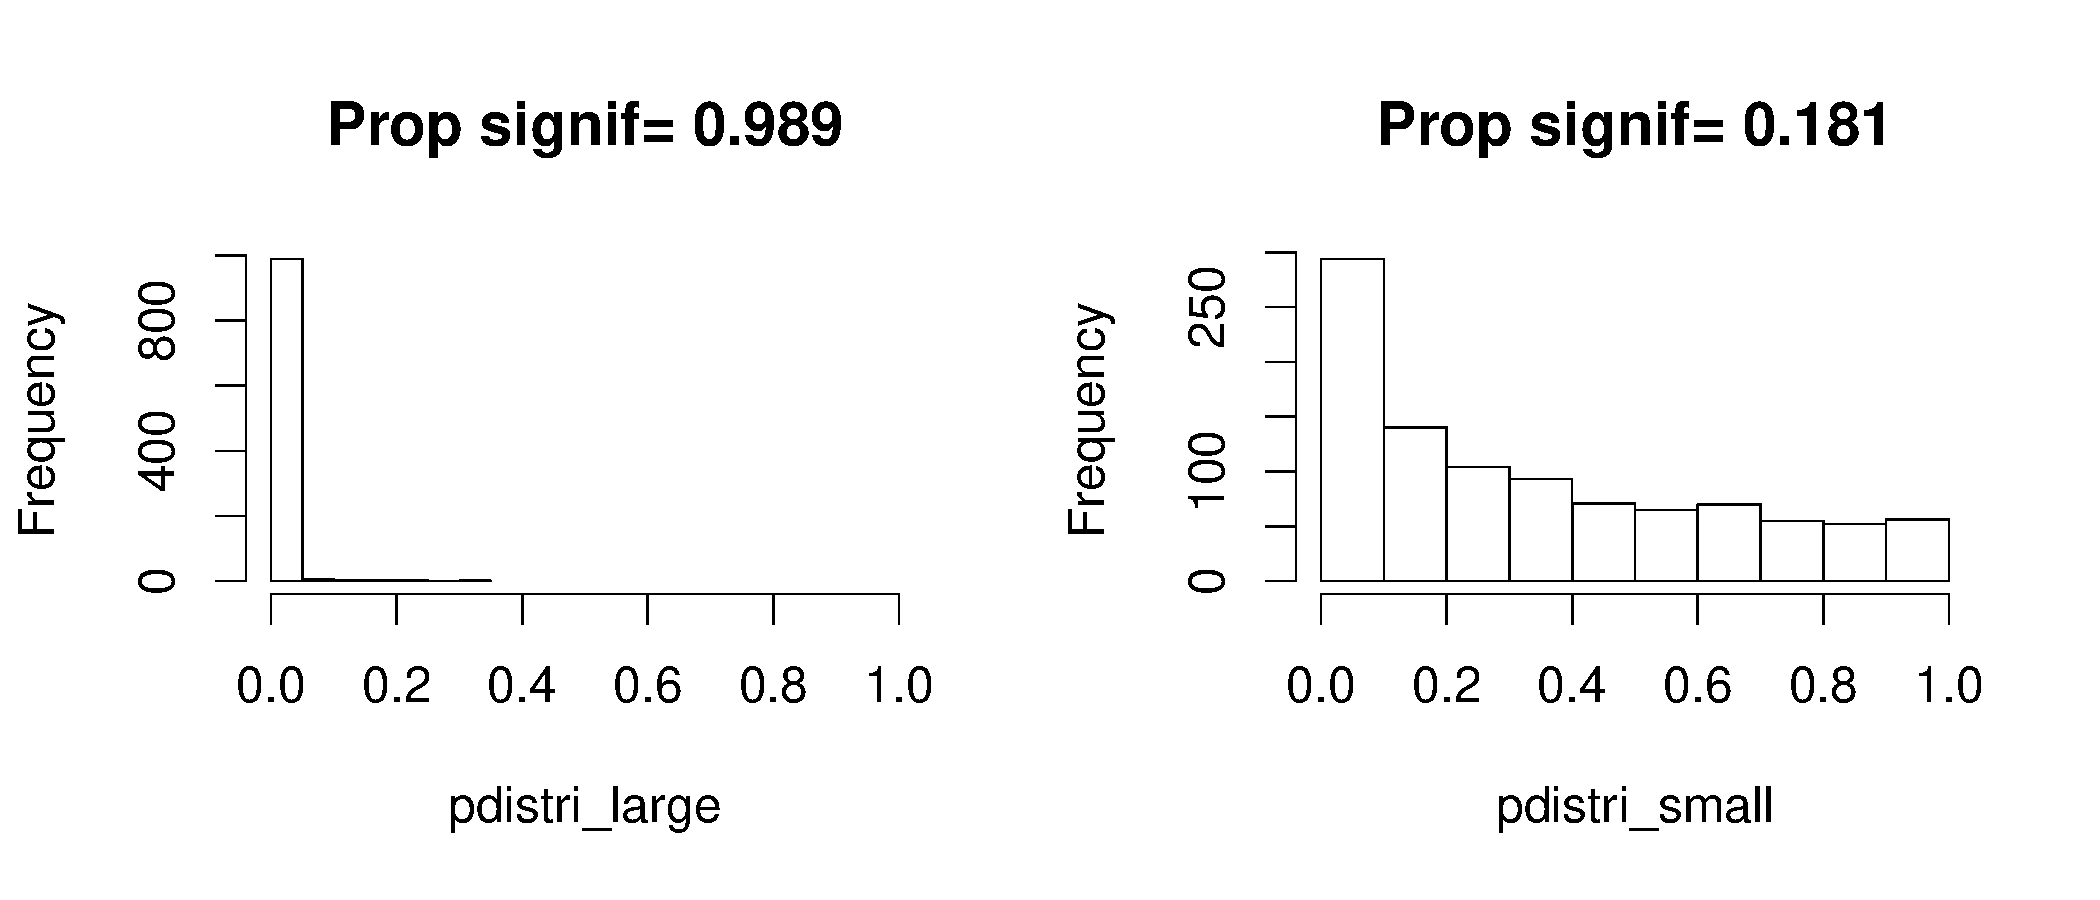
\includegraphics[width=0.8\textwidth,height=0.5\textheight]{figure/comphist1-1} 
\begin{kframe}\begin{alltt}
\hlkwd{par}\hlstd{(}\hlkwc{mfrow}\hlstd{=}\hlkwd{c}\hlstd{(}\hlnum{1}\hlstd{,}\hlnum{1}\hlstd{))}
\end{alltt}
\end{kframe}
\end{knitrout}

\end{frame}
%%%%%%%%%%%

\begin{frame}[fragile]{When do we know it is different? Try it!}

\begin{alertblock}{Exercise}
Check the effect of {\color{orange}{smaller variability}} and/or {\color{blue}{larger sample size}}.
\end{alertblock}
\end{frame}
%%%%%%%%%%%


\begin{frame}{By the way, what are these p-values?}%focus on p-value criticized

\textit{Probability for a summary statistic to be greater or equal to the observed summary statistic, \textbf{when the null-hypothesis of a given statistical model is true.}}

\pause

\begin{exampleblock}{Properties}
  \begin{itemize}
    \item Depends on the null-hypothesis ($H_0$) of a given model with assumptions
    \item Uniform distribution under $H_0$ \dots
    \item \dots hence proportion(significance under $H_0$) = significance threshold
  \end{itemize}
\end{exampleblock}

\pause
\textbf{NB: Focus on $p$-value criticized, but common and they are no more evil than other misused statistics!}
\end{frame}
%%%%%%%%%%%

\begin{frame}[fragile]{Playing with loops and p-values}

\begin{knitrout}
\definecolor{shadecolor}{rgb}{0.843, 0.867, 0.922}\color{fgcolor}\begin{kframe}
\begin{alltt}
\hlkwd{set.seed}\hlstd{(}\hlnum{1234}\hlstd{)}
\hlstd{x} \hlkwb{<-} \hlkwd{rnorm}\hlstd{(}\hlnum{100}\hlstd{)}
\hlstd{y} \hlkwb{<-} \hlkwd{rnorm}\hlstd{(}\hlnum{100}\hlstd{)}
\hlkwd{summary}\hlstd{(}\hlkwd{lm}\hlstd{(y}\hlopt{~}\hlstd{x))}
\end{alltt}
\begin{verbatim}

Call:
lm(formula = y ~ x)

Residuals:
     Min       1Q   Median       3Q      Max 
-2.88626 -0.61401  0.00236  0.58645  2.98774 

Coefficients:
            Estimate Std. Error t value Pr(>|t|)
(Intercept)  0.03715    0.10498   0.354    0.724
x           -0.02608    0.10378  -0.251    0.802

Residual standard error: 1.037 on 98 degrees of freedom
Multiple R-squared:  0.0006443,	Adjusted R-squared:  -0.009553 
F-statistic: 0.06318 on 1 and 98 DF,  p-value: 0.8021
\end{verbatim}
\end{kframe}
\end{knitrout}
\end{frame}


\begin{frame}[fragile]{Playing with loops and p-values}

\begin{alertblock}{While-loop}
Are we every going to find a significant p-value with two sets of random numbers? Write a while loop to find out. How many iterations until you find a p-value below 0.05?

\end{alertblock}

\begin{alertblock}{For-loop}
How often do you observe a significant test with randomly drawn numbers?

\end{alertblock}

\end{frame}
%%%%%%%%%%%



\section{Little R-Studio tricks}

\begin{frame}[fragile]{Column selection}

\begin{knitrout}
\definecolor{shadecolor}{rgb}{0.843, 0.867, 0.922}\color{fgcolor}\begin{kframe}
\begin{alltt}
\hlstd{lm1}   \hlkwb{<-} \hlkwd{lm}\hlstd{(y} \hlopt{~} \hlstd{x1} \hlopt{+} \hlstd{x2)}
\hlstd{lm2}   \hlkwb{<-} \hlkwd{lm}\hlstd{(y} \hlopt{~} \hlnum{1}\hlstd{)}
\hlstd{lm3}   \hlkwb{<-} \hlkwd{lm}\hlstd{(y} \hlopt{~} \hlstd{x1}\hlopt{*}\hlstd{x2)}
\hlstd{lm3}   \hlkwb{<-} \hlkwd{lm}\hlstd{(y} \hlopt{~} \hlstd{x2)}
\hlstd{lm4}   \hlkwb{<-} \hlkwd{lm}\hlstd{(y} \hlopt{~} \hlstd{x1)}
\hlstd{...}

\hlkwd{plot}\hlstd{(lm1)}
\hlkwd{plot}\hlstd{(lm2)}
\hlstd{...}
\end{alltt}
\end{kframe}
\end{knitrout}

\end{frame}
%%%%%%%%%%%

\begin{frame}[fragile]{Column selection}
You changed the name to be more explicit

\begin{knitrout}
\definecolor{shadecolor}{rgb}{0.843, 0.867, 0.922}\color{fgcolor}\begin{kframe}
\begin{alltt}
\hlstd{lmadd}  \hlkwb{<-} \hlkwd{lm}\hlstd{(y} \hlopt{~} \hlstd{x1} \hlopt{+} \hlstd{x2)}
\hlstd{lmnull} \hlkwb{<-} \hlkwd{lm}\hlstd{(y} \hlopt{~} \hlnum{1}\hlstd{)}
\hlstd{lmff}   \hlkwb{<-} \hlkwd{lm}\hlstd{(y} \hlopt{~} \hlstd{x1}\hlopt{*}\hlstd{x2)}
\hlstd{lmx2}   \hlkwb{<-} \hlkwd{lm}\hlstd{(y} \hlopt{~} \hlstd{x2)}
\hlstd{lmx1}   \hlkwb{<-} \hlkwd{lm}\hlstd{(y} \hlopt{~} \hlstd{x1)}
\hlstd{...}

\hlkwd{plot}\hlstd{(lm1)}
\hlkwd{plot}\hlstd{(lm2)}
\hlstd{...}
\end{alltt}
\end{kframe}
\end{knitrout}

What a pain to repeat the changes in \texttt{plot()}!
\pause

\color{blue}{\texttt{Alt + click}}
\end{frame}
%%%%%%%%%%%%


\begin{frame}[fragile]{Column selection}
What if my code was not well aligned??

\begin{knitrout}
\definecolor{shadecolor}{rgb}{0.843, 0.867, 0.922}\color{fgcolor}\begin{kframe}
\begin{alltt}
\hlstd{lmadd} \hlkwb{<-} \hlkwd{lm}\hlstd{(y} \hlopt{~} \hlstd{x1} \hlopt{+} \hlstd{x2)}
\hlstd{lmnull} \hlkwb{<-} \hlkwd{lm}\hlstd{(y} \hlopt{~} \hlnum{1}\hlstd{)}
\hlstd{lmff} \hlkwb{<-} \hlkwd{lm}\hlstd{(y} \hlopt{~} \hlstd{x1}\hlopt{*}\hlstd{x2)}
\hlstd{lmx2}\hlkwb{<-} \hlkwd{lm}\hlstd{(y} \hlopt{~} \hlstd{x2)}
\hlstd{lmx1}  \hlkwb{<-} \hlkwd{lm}\hlstd{(y} \hlopt{~} \hlstd{x1)}
\hlstd{...}

\hlkwd{plot}\hlstd{(lm1)}
\hlkwd{plot}\hlstd{(lm2)}
\hlstd{...}
\end{alltt}
\end{kframe}
\end{knitrout}

\pause

\color{blue}{\texttt{Ctrl + Alt + clicks}} creates multiple cursors\\

then \color{blue}{\texttt{Shift + Home}} and \texttt{Ctrl + C}
\end{frame}
%%%%%%%%%%%%


\begin{frame}{Shortcuts}

\color{blue}{\texttt{Alt + Shift + K}}

\end{frame}
%%%%%%%%%%%%

\section{t-test, ANOVA, regression: all is one, one is all}

\begin{frame}[fragile]{A small example}

Animal behavior in response to weather



Load data:
\begin{knitrout}
\definecolor{shadecolor}{rgb}{0.843, 0.867, 0.922}\color{fgcolor}\begin{kframe}
\begin{alltt}
\hlkwd{getwd}\hlstd{()}
\hlkwd{setwd}\hlstd{()}
\end{alltt}
\end{kframe}
\end{knitrout}

\begin{knitrout}
\definecolor{shadecolor}{rgb}{0.843, 0.867, 0.922}\color{fgcolor}\begin{kframe}
\begin{alltt}
\hlstd{dat.behav} \hlkwb{<-} \hlkwd{read.csv}\hlstd{(}\hlkwc{file} \hlstd{=} \hlstr{"Data/datbehav.csv"}\hlstd{)} \hlcom{# path to file}
\end{alltt}
\end{kframe}
\end{knitrout}

\pause
STEP 1: have a look at your data
\begin{knitrout}
\definecolor{shadecolor}{rgb}{0.843, 0.867, 0.922}\color{fgcolor}\begin{kframe}
\begin{alltt}
\hlkwd{str}\hlstd{(dat.behav)}
\hlkwd{summary}\hlstd{(dat.behav)}
\hlkwd{plot}\hlstd{(dat.behav)}
\end{alltt}
\end{kframe}
\end{knitrout}
\end{frame}
%%%%%%%%%%%%%%%%%%%%%%

\begin{frame}[fragile]{t-test}
\begin{knitrout}
\definecolor{shadecolor}{rgb}{0.843, 0.867, 0.922}\color{fgcolor}\begin{kframe}
\begin{alltt}
\hlstd{fitstudent} \hlkwb{<-} \hlkwd{t.test}\hlstd{(}\hlkwc{x} \hlstd{= dat.behav}\hlopt{$}\hlstd{activity[dat.behav}\hlopt{$}\hlstd{weather}\hlopt{==}
                                              \hlstr{"rainy"}\hlstd{],}
                     \hlkwc{y} \hlstd{= dat.behav}\hlopt{$}\hlstd{activity[dat.behav}\hlopt{$}\hlstd{weather}\hlopt{==}
                                              \hlstr{"sunny"}\hlstd{],}
                     \hlkwc{var.equal} \hlstd{=} \hlnum{TRUE}\hlstd{)}
\hlkwd{print}\hlstd{(fitstudent)}
\end{alltt}
\begin{verbatim}

	Two Sample t-test

data:  dat.behav$activity[dat.behav$weather == "rainy"] and dat.behav$activity[dat.behav$weather == "sunny"]
t = 3.2752, df = 33, p-value = 0.002485
alternative hypothesis: true difference in means is not equal to 0
95 percent confidence interval:
 0.6138373 2.6270325
sample estimates:
mean of x mean of y 
 6.781476  5.161041 
\end{verbatim}
\end{kframe}
\end{knitrout}
\end{frame}
%%%%%%%%%%%

\begin{frame}[fragile]{t-test, graphically}
\textbf{Difference between means}
\centering
\begin{knitrout}
\definecolor{shadecolor}{rgb}{0.843, 0.867, 0.922}\color{fgcolor}
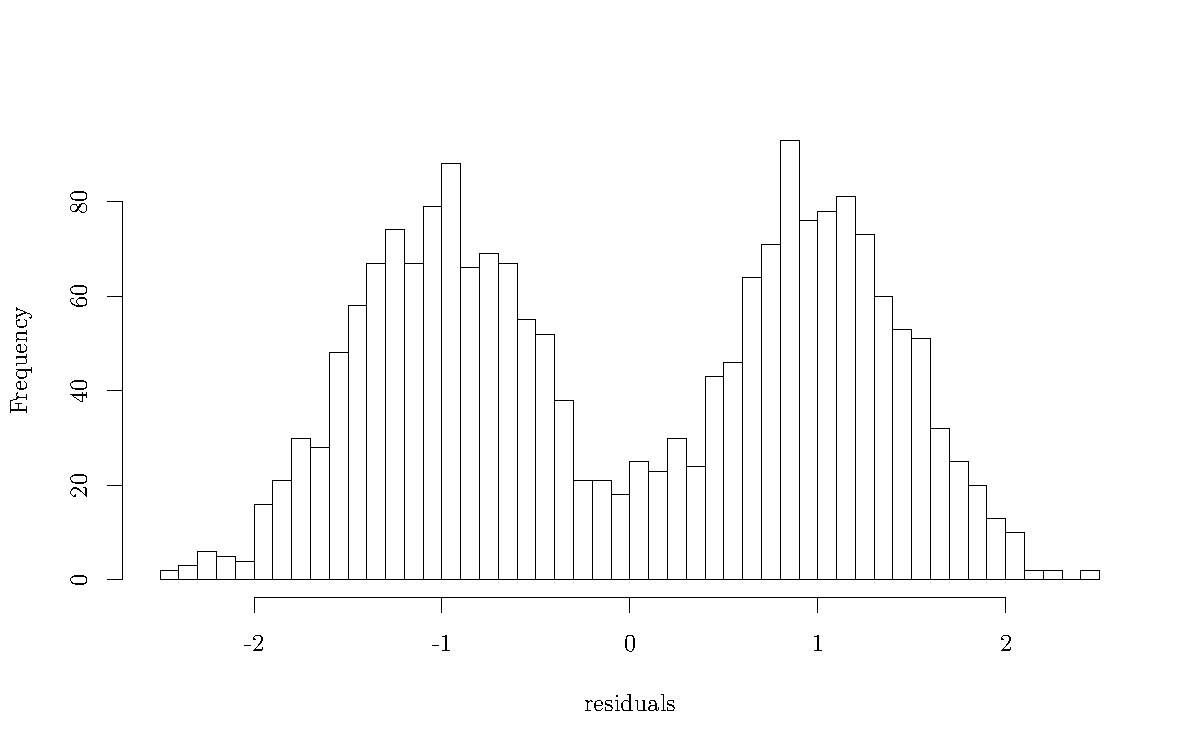
\includegraphics[width=0.8\textwidth,height=0.6\textwidth]{figure/unnamed-chunk-15-1} 

\end{knitrout}
\end{frame}
%%%%%%%%%%

\begin{frame}[fragile]{ANOVA}  \begin{enumerate}
    \item What is the fastest way to get row averages in a data-frame?
    \item Create a function called colVars, like colMeans but for variance
    \item Create nice plots to visualize iris data (ideally journal-quality)
  \end{enumerate}


\begin{knitrout}
\definecolor{shadecolor}{rgb}{0.843, 0.867, 0.922}\color{fgcolor}\begin{kframe}
\begin{alltt}
\hlstd{fitanova} \hlkwb{<-} \hlkwd{aov}\hlstd{(}\hlkwc{data} \hlstd{= dat.behav,} \hlkwc{formula} \hlstd{= activity} \hlopt{~} \hlstd{weather)}
\hlkwd{summary}\hlstd{(fitanova)}
\end{alltt}
\begin{verbatim}
            Df Sum Sq Mean Sq F value  Pr(>F)   
weather      1  11.25  11.253   10.73 0.00248 **
Residuals   33  34.62   1.049                   
---
Signif. codes:  0 '***' 0.001 '**' 0.01 '*' 0.05 '.' 0.1 ' ' 1
\end{verbatim}
\end{kframe}
\end{knitrout}
\end{frame}
%%%%%%%%%%%

\begin{frame}[fragile]{ANOVA, graphically}
\textbf{Variance decomposition}
\centering
\begin{knitrout}
\definecolor{shadecolor}{rgb}{0.843, 0.867, 0.922}\color{fgcolor}
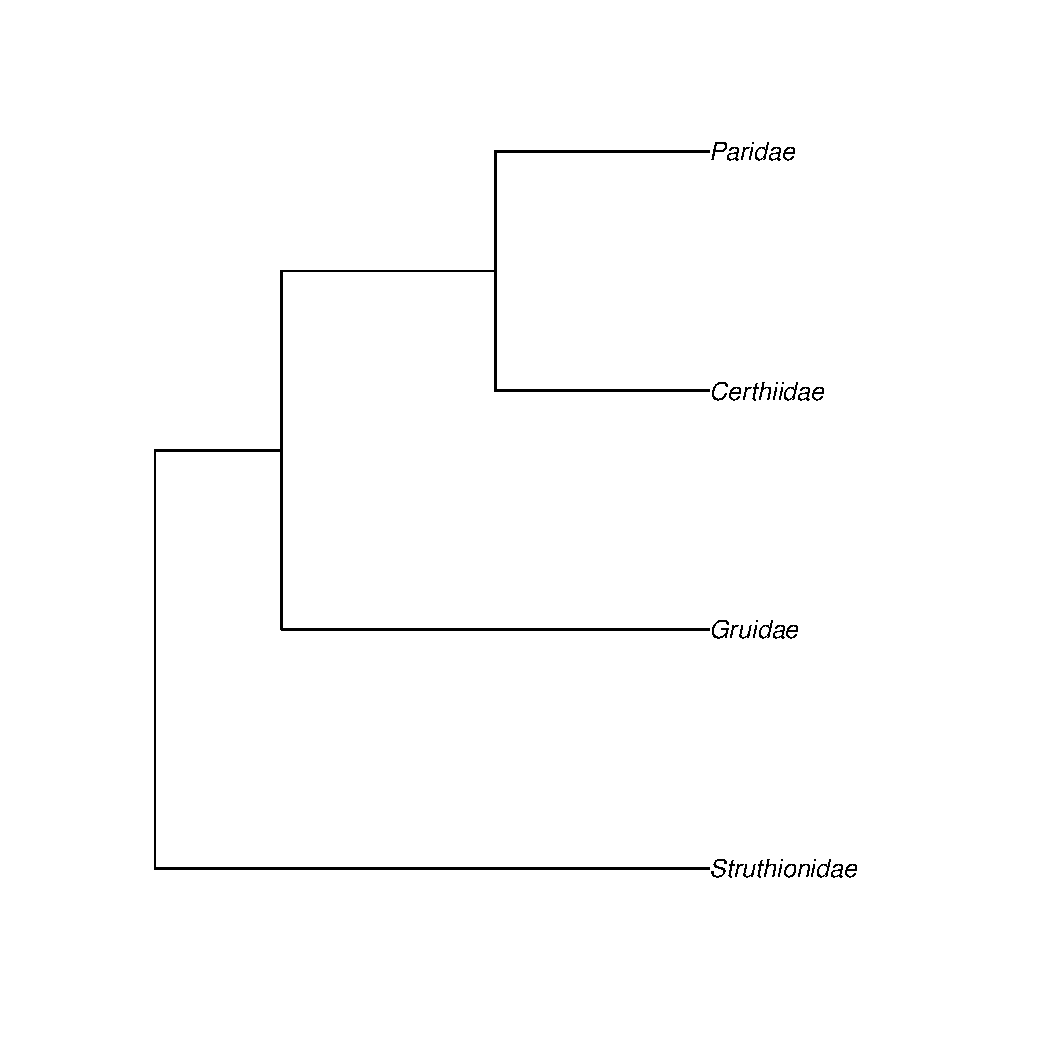
\includegraphics[width=0.8\textwidth,height=0.6\textwidth]{figure/unnamed-chunk-17-1} 

\end{knitrout}
\end{frame}
%%%%%%%%%%

\begin{frame}[fragile]{Linear regression}

\begin{knitrout}
\definecolor{shadecolor}{rgb}{0.843, 0.867, 0.922}\color{fgcolor}\begin{kframe}
\begin{alltt}
\hlstd{fitlm} \hlkwb{<-} \hlkwd{lm}\hlstd{(}\hlkwc{data} \hlstd{= dat.behav,} \hlkwc{formula} \hlstd{= activity} \hlopt{~} \hlstd{weather)}
\hlkwd{summary}\hlstd{(fitlm)}
\end{alltt}
\begin{verbatim}

Call:
lm(formula = activity ~ weather, data = dat.behav)

Residuals:
    Min      1Q  Median      3Q     Max 
-2.3547 -0.6028  0.2346  0.6419  1.6534 

Coefficients:
             Estimate Std. Error t value Pr(>|t|)    
(Intercept)    6.7815     0.4581  14.805 3.94e-16 ***
weathersunny  -1.6204     0.4948  -3.275  0.00248 ** 
---
Signif. codes:  0 '***' 0.001 '**' 0.01 '*' 0.05 '.' 0.1 ' ' 1

Residual standard error: 1.024 on 33 degrees of freedom
Multiple R-squared:  0.2453,	Adjusted R-squared:  0.2224 
F-statistic: 10.73 on 1 and 33 DF,  p-value: 0.002485
\end{verbatim}
\end{kframe}
\end{knitrout}
\end{frame}
%%%%%%%%%%%

\begin{frame}[fragile]{Regression, graphically}
\textbf{Rate of change}
\centering
\begin{knitrout}
\definecolor{shadecolor}{rgb}{0.843, 0.867, 0.922}\color{fgcolor}
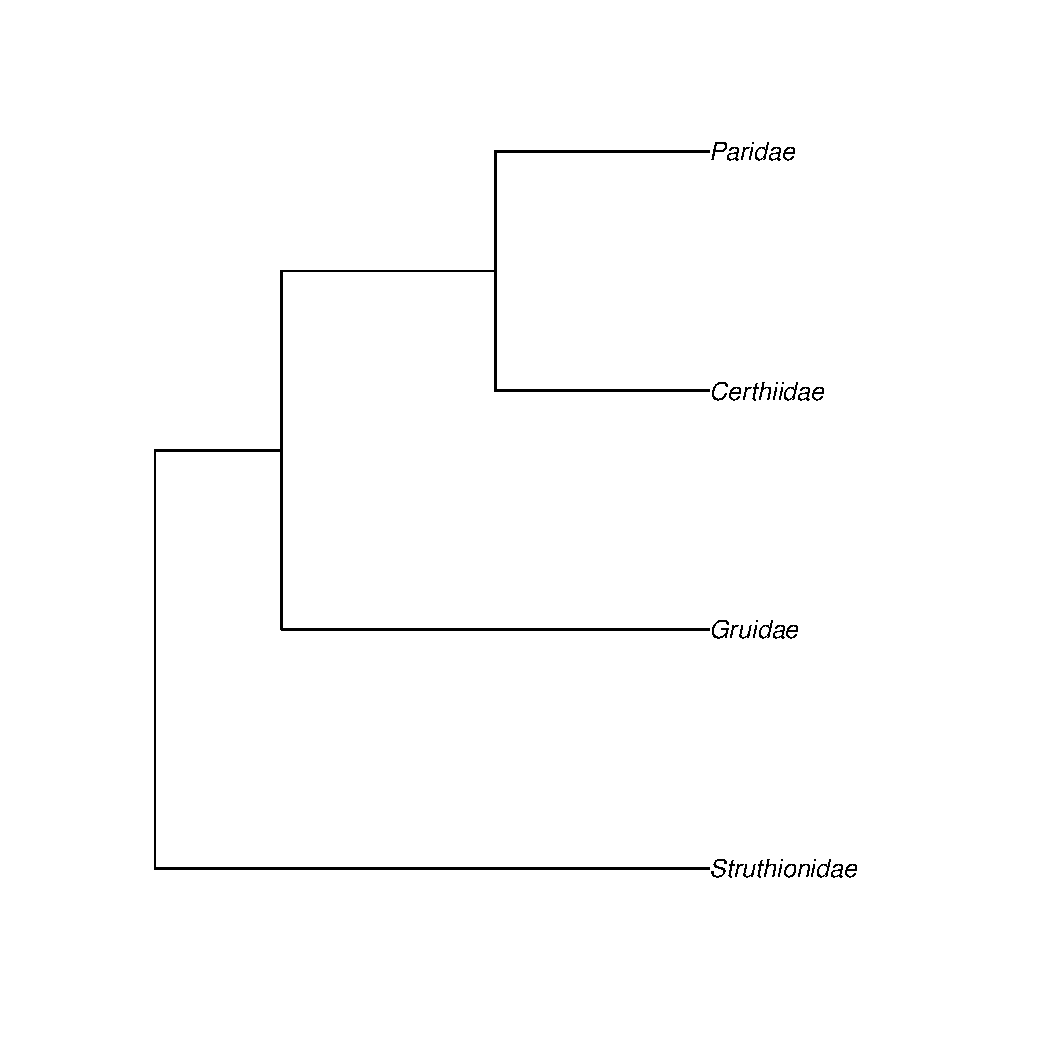
\includegraphics[width=0.8\textwidth,height=0.6\textwidth]{figure/unnamed-chunk-19-1} 

\end{knitrout}
\end{frame}
%%%%%%%%%%


\begin{frame}[fragile]{NB: aov() vs. anova()}

\begin{knitrout}
\definecolor{shadecolor}{rgb}{0.843, 0.867, 0.922}\color{fgcolor}\begin{kframe}
\begin{alltt}
\hlkwd{aov}\hlstd{(}\hlkwc{data} \hlstd{= dat.behav,} \hlkwc{formula} \hlstd{= activity} \hlopt{~} \hlstd{weather)}
\hlkwd{anova}\hlstd{(fitlm)}
\end{alltt}
\end{kframe}
\end{knitrout}

\end{frame}
%%%%%%%%%%%

\begin{frame}{All is one\dots}
\pause
  \begin{block}{\dots but \texttt{lm()} rules!}
    \begin{itemize}
      \item t-test, ANOVA, regression and others can be mathematically equivalent
      \item In R, \texttt{lm()} and related functions can do them all\dots
      \item \dots and much more!
    \end{itemize}
  \end{block}
\end{frame}
%%%%%%%%%%%

%%%%%%%%%%%%%%%%%%%%%%%%%%%%%%%%%%%%%%%%%%%%%%%%%%%%%%%%%%%%%%%%%%%
%%%%%%%%%%%%%%%%%%%%%%%%%%%%%%%%%%%%%%%%%%%%%%%%%%%%%%%%%%%%%%%%%%%
\section{Linear models in details}

\begin{frame}[fragile]{A simple linear model}
  \textbf{{\color{purple}{Response}} = {\color{blue}{Intercept}} + {\color{red}{Slope}} $\times$ {\color{orange}{Predictor}} + {\color{gray}{Error}}} \\
  
\begin{knitrout}
\definecolor{shadecolor}{rgb}{0.843, 0.867, 0.922}\color{fgcolor}
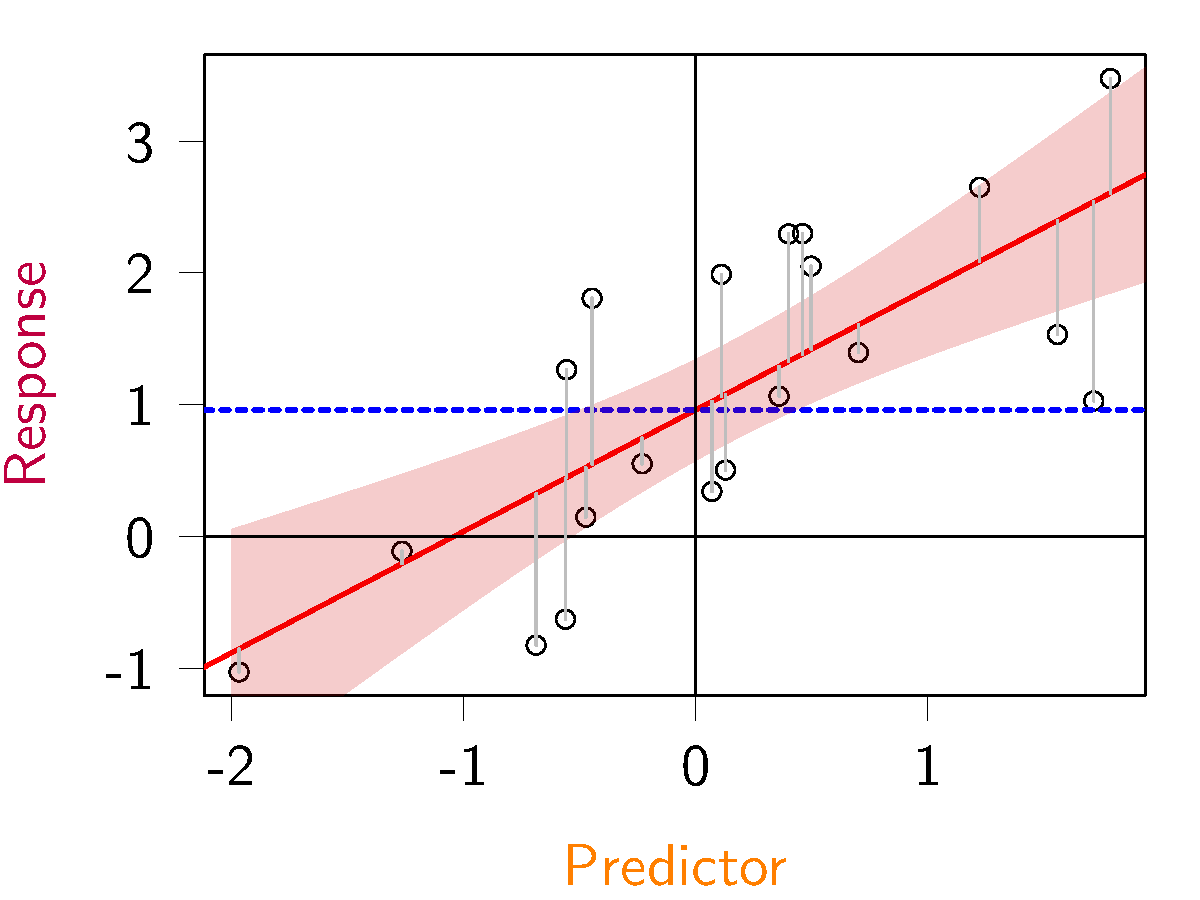
\includegraphics[width=0.8\textwidth,height=0.6\textwidth]{figure/lmprinc-1} 

\end{knitrout}
\end{frame}
%%%%%%%%%%%

\begin{frame}[fragile]{A simple linear model}
  \textbf{{\color{purple}{Response}} = {\color{blue}{Intercept}} + {\color{red}{Slope}} $\times$ {\color{orange}{Predictor}} + {\color{gray}{Error}}} \\
  \vspace{1cm}
\textbf{In R:}
\begin{knitrout}
\definecolor{shadecolor}{rgb}{0.843, 0.867, 0.922}\color{fgcolor}\begin{kframe}
\begin{alltt}
  \hlkwd{lm}\hlstd{(response} \hlopt{~} \hlnum{1} \hlopt{+} \hlstd{predictor1} \hlopt{+} \hlstd{predictor2,} \hlkwc{data}\hlstd{=data)}
    \hlcom{# equivalent to}
  \hlkwd{lm}\hlstd{(response} \hlopt{~} \hlstd{predictor1} \hlopt{+} \hlstd{predictor2,} \hlkwc{data}\hlstd{=data)}
\end{alltt}
\end{kframe}
\end{knitrout}
\begin{itemize}
  \item Intercept can be explicit or implicit
  \item Can remove intercept with \texttt{\dots $\sim $ 0 + \dots}
  \item Error is implicit
  \item Feed the option \texttt{data=} to keep code short, reliable and flexible
  \item Order of predictors do not matter 
\end{itemize}

\end{frame}
%%%%%%%%%%%

\begin{frame}[fragile]{Interpretation}

\begin{knitrout}
\definecolor{shadecolor}{rgb}{0.843, 0.867, 0.922}\color{fgcolor}\begin{kframe}
\begin{alltt}
  \hlstd{Ans} \hlkwb{<-} \hlkwd{read.csv}\hlstd{(}\hlkwc{file} \hlstd{=} \hlstr{"Data/Anscombe.csv"}\hlstd{)}
\end{alltt}
\end{kframe}
\end{knitrout}
  
\begin{knitrout}
\definecolor{shadecolor}{rgb}{0.843, 0.867, 0.922}\color{fgcolor}\begin{kframe}
\begin{alltt}
  \hlstd{lm1} \hlkwb{<-} \hlkwd{lm}\hlstd{(y} \hlopt{~} \hlstd{x ,} \hlkwc{data}\hlstd{=Ans[Ans}\hlopt{$}\hlstd{distri}\hlopt{==}\hlnum{1}\hlstd{,])}
  \hlkwd{summary}\hlstd{(lm1)}
  \hlkwd{plot}\hlstd{(Ans}\hlopt{$}\hlstd{x[Ans}\hlopt{$}\hlstd{distri}\hlopt{==}\hlnum{1}\hlstd{], Ans}\hlopt{$}\hlstd{y[Ans}\hlopt{$}\hlstd{distri}\hlopt{==}\hlnum{1}\hlstd{],}
       \hlkwc{xlim}\hlstd{=}\hlkwd{c}\hlstd{(}\hlnum{0}\hlstd{,}\hlnum{15}\hlstd{),} \hlkwc{ylim}\hlstd{=}\hlkwd{c}\hlstd{(}\hlnum{0}\hlstd{,}\hlnum{12}\hlstd{))}
  \hlkwd{abline}\hlstd{(lm1)}
\end{alltt}
\end{kframe}
\end{knitrout}
\end{frame}
%%%%%%%%%%%

\begin{frame}[fragile]{Interpretation}

 \begin{alertblock}{lm vs. plot}
 \begin{itemize}
   \item Fit a linear model $y \sim x$for each of the four ``distri"
   \item Plot the relationship  $ y \sim x $ for each of the four ``distri"
   \item Can we trust these models? For what? 
  \end{itemize}
 \end{alertblock}

\end{frame}
%%%%%%%%%%%

\begin{frame}{General approach}

\begin{center}
  \begin{tikzpicture}
    \node (sq) at (0,-1) {\color{red}{1. Scientific question}};
    \node (mo) at (0,-2) {2. Model and Statistical question};
    \draw[->, thick] (sq)--(mo);
    \node (dac) at (6,-2) {\color{red}{3. Data collection}};
    \draw[<->, thick] (mo)--(dac);

    \node (est) at (0,-3) {4. Estimation};
        \draw[->, thick] (mo)--(est);
    \node (unc) at (0,-3.5) {4.b Uncertainty and statistical significance};
    
    \node (che) at (0,-5) {\textbf{5. Diagnostic, check assumptions, prediction}};
        \draw[->, thick] (unc)--(che);
    \draw[->, thick] (che.west) to [out=150, in=210] (mo.west);

    \node (int) at (0,-6) {\color{red}{6. Interpret and think about the biology}};
        \draw[->, thick] (che)--(int);

  \draw[rounded corners, color=blue] (-4.5,-1.5) rectangle (4,-5.5);
  \node[anchor=north west] (r) at (-4.5,-1.5) {
\includegraphics[width=0.1\textwidth]{Figures/r}};
  \end{tikzpicture}
  \end{center}
\end{frame}
%%%%%%%%%%%

\begin{frame}{Linear model basic assumptions}
Not necessarily wrong, but typical interpretation assumes:
 \begin{block}{}
     \begin{itemize}[<+->]
      \item Linear combination of parameters (including transformation, polynoms, interactions\dots)\\ \textit{Risk: biologically meaningless}
      \item Predictor not perfectly correlated \\ \textit{Risk: Model won't run, unstable convergence, or huge SE}
       \item {\color{red!20!black}{Little error in predictors}}\\ \textit{Risk: bias estimates (underestimate with Gaussian error)}
       \item {\color{red!50!black}{Gaussian error distribution}}\\ \textit{Risk: Poor predictions}
       \item {\color{red!70!black}{Homoscedasticity (constant error variance)}}\\ \textit{Risk: Over-optimistic uncertainty, unreliable predictions}
       \item {\color{red!99!black}{Independence of error}}\\ \textit{Risk: Bias and over-optimistic uncertainty}
     \end{itemize}
 \end{block}
\end{frame}
%%%%%%%%%%%

\begin{frame}[fragile]{Diagnostic: summary and plot}
\begin{knitrout}
\definecolor{shadecolor}{rgb}{0.843, 0.867, 0.922}\color{fgcolor}\begin{kframe}
\begin{alltt}
 \hlstd{lm1} \hlkwb{<-} \hlkwd{lm}\hlstd{(y} \hlopt{~} \hlstd{x ,} \hlkwc{data}\hlstd{=Ans[Ans}\hlopt{$}\hlstd{distri}\hlopt{==}\hlnum{1}\hlstd{,])}
 \hlstd{lm2} \hlkwb{<-} \hlkwd{lm}\hlstd{(y} \hlopt{~} \hlstd{x ,} \hlkwc{data}\hlstd{=Ans[Ans}\hlopt{$}\hlstd{distri}\hlopt{==}\hlnum{2}\hlstd{,])}
\end{alltt}
\end{kframe}
\end{knitrout}
  
  
\begin{knitrout}
\definecolor{shadecolor}{rgb}{0.843, 0.867, 0.922}\color{fgcolor}\begin{kframe}
\begin{alltt}
 \hlkwd{summary}\hlstd{(lm1)}
 \hlkwd{par}\hlstd{(}\hlkwc{mfrow}\hlstd{=}\hlkwd{c}\hlstd{(}\hlnum{2}\hlstd{,}\hlnum{2}\hlstd{))}
 \hlkwd{plot}\hlstd{(lm1)}
\end{alltt}
\end{kframe}
\end{knitrout}
  
\begin{knitrout}
\definecolor{shadecolor}{rgb}{0.843, 0.867, 0.922}\color{fgcolor}\begin{kframe}
\begin{alltt}
  \hlkwd{summary}\hlstd{(lm2)}
 \hlkwd{plot}\hlstd{(lm2)}
  \hlkwd{par}\hlstd{(}\hlkwc{mfrow}\hlstd{=}\hlkwd{c}\hlstd{(}\hlnum{1}\hlstd{,}\hlnum{1}\hlstd{))}
\end{alltt}
\end{kframe}
\end{knitrout}

\end{frame}

\begin{frame}[fragile]{Diagnostic: prediction}
\begin{knitrout}
\definecolor{shadecolor}{rgb}{0.843, 0.867, 0.922}\color{fgcolor}\begin{kframe}
\begin{alltt}
\hlstd{pred2} \hlkwb{<-} \hlkwd{predict}\hlstd{(lm2,} \hlkwc{se.fit} \hlstd{=} \hlnum{TRUE}\hlstd{,} \hlkwc{interval} \hlstd{=} \hlstr{"confidence"}\hlstd{)}
\hlstd{pred2} \hlkwb{<-} \hlkwd{cbind}\hlstd{(Ans[Ans}\hlopt{$}\hlstd{distri}\hlopt{==}\hlnum{2}\hlstd{,], pred2)}
\end{alltt}
\end{kframe}
\end{knitrout}

\pause
\begin{knitrout}
\definecolor{shadecolor}{rgb}{0.843, 0.867, 0.922}\color{fgcolor}
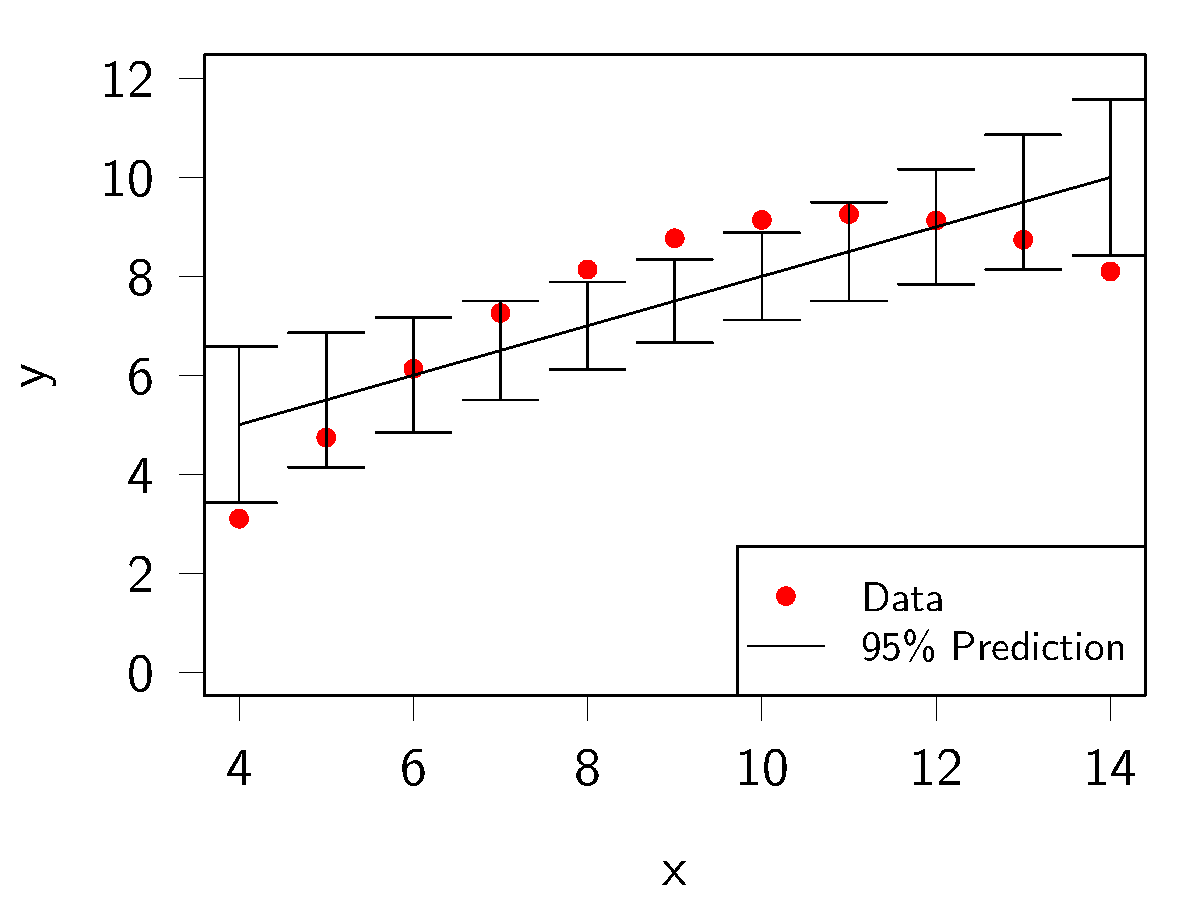
\includegraphics[width=0.8\textwidth,height=0.6\textwidth]{figure/pred2-1} 

\end{knitrout}
\end{frame}
%%%%%%%%%%%

\begin{frame}[fragile]{Practice lm() with parasites}


  
  \begin{alertblock}{What explains variation in parasitic load?}
  You collected ecto-parasites on some furry large mammals at three locations. Parasites break easily when we collect them and are impossible to count, so we decide to measure parasitic load as their mass. \textbf{Why do some mammals have larger parasitic load?} \pause
    \begin{itemize}
      \item Load the \texttt{Para.csv} data (don't forget: str(), summary(), plot()\dots)
      \item Model \verb+Parasite_Mass+ using \texttt{lm()}
      \item Find what variables predict \verb+Parasite_Mass+
      \item How good are your models? Assumptions? Prediction?
      \item What biological interpretation can you imagine?
      \end{itemize}
  \end{alertblock}
  
\end{frame}
%%%%%%%%%%%%%%%%%%%%%%%%%%%%%%%%%%%%%%%%%%%%%%%%%%%%%%%%%%%%%%%%%%%%%%%%%%%%%%%%%


\end{document}
